\documentclass[11pt,a4paper]{article}

% ---------------------------------------------------------------
% Packages
% ---------------------------------------------------------------
\usepackage[utf8]{inputenc}
\usepackage[T1]{fontenc}
\usepackage{lmodern}
\usepackage{amsmath}
\usepackage[margin=2.2cm]{geometry}
\usepackage{graphicx}
\usepackage{booktabs}
\usepackage{tabularx}
\usepackage{xcolor}
\usepackage{listings}
\usepackage{caption}
\usepackage{subcaption}
\usepackage{enumitem}
\usepackage{microtype}
\usepackage[hidelinks]{hyperref}

\graphicspath{{figures/}}
\setlist{nosep, leftmargin=*}
\setlength{\parskip}{0.4em}
\setlength{\parindent}{0pt}
\setlength{\emergencystretch}{3em}  % long \code{} paths: move to the next line instead of overflowing
\captionsetup{font=small, labelfont=bf}

\definecolor{codebg}{gray}{0.96}
\definecolor{codecomment}{rgb}{0.35,0.45,0.35}
\definecolor{codekw}{rgb}{0.10,0.25,0.55}
\lstset{
  language=Python,
  basicstyle=\ttfamily\footnotesize,
  backgroundcolor=\color{codebg},
  keywordstyle=\color{codekw}\bfseries,
  commentstyle=\color{codecomment}\itshape,
  stringstyle=\color{black!70},
  frame=single, rulecolor=\color{black!20},
  breaklines=true, columns=fullflexible,
  showstringspaces=false,
  xleftmargin=2pt, xrightmargin=2pt,
  aboveskip=0.6em, belowskip=0.4em
}

\newcommand{\code}[1]{\texttt{#1}}

% ---------------------------------------------------------------
\title{\textbf{Rogaland Transit Medallion}\\[0.3em]
\large How punctual are the buses in Rogaland?\\[0.5em]
\normalsize DAT535 Data Engineering, Group 5}
\author{Tommaso Facchin \and Oliwier Trawinski}
\date{University of Stavanger, November 2026}

\begin{document}
\maketitle

\begin{abstract}
\noindent
Entur publishes live trip updates for all Kolumbus buses and boats in Rogaland, but the
API only shows the current state and keeps no history. To find out which lines, stops and
hours are late most often, we poll the SIRI ET feed every 5 minutes and build the history
ourselves. Bronze keeps every raw response. Silver turns about 3.4 million repeated stop
observations per day into roughly 153{,}000 stop calls, and Gold aggregates them into two
punctuality tables. Everything runs on two OpenStack VMs with PySpark, and GitHub Actions
handles tests, deployment and the nightly run. The pipeline has collected data since
27 October 2026. About 55\% of stops are on time, 15:00 is the worst hour (33\%) and X39
the worst line (15\%).
\end{abstract}

\section{Scope}

The question we want to answer is which Kolumbus lines, stops and hours in Rogaland are
least punctual. A planner at Kolumbus or the county could use the answer to decide where
to fix timetables first. We picked this data because we take these buses every day, and
because it forces some real decisions: there is no historical download, so collection had
to work from the first day, and every snapshot repeats all running trips, so most of the
Silver work is deduplication.

We left out streaming (a nightly batch is enough for this question), trips that never show
up in the feed (that would need the GTFS timetable), passenger numbers and a finished
dashboard.

The course suggests one notebook per layer. We kept the three layers but wrote them as
Python modules (\code{bronze/}, \code{silver/}, \code{gold/}) with one entry point,
\code{jobs/run\_pipeline.py}, because we wanted to schedule the pipeline every night and
unit test it, and both are much easier with modules.

\section{The data}

The source is Entur's real-time API, SIRI Estimated Timetable
(\code{/realtime/v1/rest/}\allowbreak\code{et?datasetId=KOL}). No key is needed, only an
\code{ET-Client-Name} header and a polite request rate. The data is open under NLOD.
\code{datasetId=KOL} returned 679 trips, all Kolumbus; \code{datasource=KOL} did not filter
anything. One response is an XML file of about 9\,MB with every running trip. Inside it, an
\code{EstimatedVehicleJourney} is one trip, with its \code{RecordedCall}s (stops already
passed, real times) and \code{EstimatedCall}s (stops ahead, predictions).

We looked at raw snapshots for a few days before designing anything, and found these
problems:
\begin{itemize}
  \item times have a local offset (\code{+01:00}), and daylight saving changed on 25 Oct;
  \item the same stop is repeated in about 22 snapshots in a row;
  \item \code{PublishedLineName} is empty, so lines are only ids like \code{KOL:Line:8\_2043};
  \item \code{Cancellation} is usually left out instead of being false;
  \item some stop names have broken encoding (\code{Ã} instead of \code{ø});
  \item one line can have several route variants (X39 has three).
\end{itemize}

At one snapshot every 5 minutes this is 288 files and 2.6\,GB a day before compression.
A Silver run reads 864 files (Section~\ref{sec:silver}) and the archive grows every day,
and the work splits naturally per file, so Spark is a reasonable fit even though the final
tables are small.

\section{Setup}

We have two OpenStack VMs, \code{dat535-dev} and \code{dat535-prod}, with 8\,GB RAM each.
There is only one floating IP, so prod has it and we reach dev through prod with SSH
ProxyJump. Prod has a 200\,GB volume on \code{/data} so the data is not on the system disk
and survives a rebuilt VM. Both VMs have a self-hosted GitHub runner. Dev and prod run the
same code; only the config file differs (data folder, client name). Spark 4.1.3 runs in
local mode with a 4\,GB driver, so the executors are the cores of the VM.

The flow is: cron on prod saves a Bronze snapshot every 5 minutes. Every night a GitHub
Actions workflow on the prod runner builds Silver for the day before, updates the line
names, and builds Gold.

\section{Bronze}

Because the API has no history, the polling interval decides what we can ever know. On
26 Oct we saved 32 snapshots 5 minutes apart on dev and checked, for every trip, the last
snapshot it was still in against the time of its last stop
(\code{scripts/retention\_check.py}). Finished trips stayed 4 to 11 minutes and were gone
after about 13. With 15 minutes we would lose the final real times of most trips, so we
poll every 5 minutes.

At first we also had a 5-minute schedule in GitHub Actions. Together with cron this fetched
every snapshot twice on 27 Oct, and GitHub's scheduled runs were often late anyway. We
removed it. Cron runs \code{scripts/run\_bronze\_cron.sh} with \code{flock -n}, so two runs
can never overlap.

Each response is saved exactly as received, gzipped, in
\code{bronze/entur\_siri/}\allowbreak\code{dt=YYYY-MM-DD/}\allowbreak\code{hour=HH/}, with
the \code{run\_id} in the file name. Gzip is lossless and makes the files about 15 times
smaller (85\,MB a day), and both Python and Spark read \code{.gz} directly. Folders use UTC
so daylight saving cannot create a missing or doubled hour.

Every run, failed or not, also writes one JSON line of metadata: time, HTTP status, size,
SHA-256 and error. The request is retried 3 times. If the XML is broken we still save it and
mark it \code{parse\_error}; Silver decides later what to skip. Files are written under a
\code{\_tmp\_} name and then renamed with \code{os.replace}, which is atomic, so a crash
cannot leave half a file behind. An existing file is never overwritten. Since every Silver
row keeps its \code{run\_id}, any number can be traced back to one Bronze file.
\code{jobs/bronze\_summary.py} reads the metadata with Spark and reports runs per day and
gaps (Figure~\ref{fig:bronze}).

\section{Silver}
\label{sec:silver}

\subsection{Grain and parsing}

One Silver row is one stop of one trip on one service date, with the key
\code{journey\_id + service\_date + stop\_order}. That is the smallest unit where
punctuality makes sense, and it keeps Silver useful for other questions than ours.
\code{service\_date} comes from \code{DataFrameRef} in the feed, not from the clock, so a
trip at 00:30 belongs to the right operating day. Silver also computes the arrival and
departure delay in seconds (actual or expected minus aimed), and keeps \code{snapshot\_time},
\code{run\_id} and \code{call\_status} (recorded or estimated). The data dictionary in the
repo lists every column with how often it is filled.

We tried Spark's XML reader first. It dropped the \code{+01:00} from the timestamps, which
would have shifted every delay by an hour without any error, and it gave recorded and
estimated stops different structures. So \code{flatten.py} parses each file with
ElementTree and \code{standardize.py} converts all times to UTC. Spark still spreads the
files over tasks:

\begin{lstlisting}[caption={Reading Bronze in \code{silver/build.py} (shortened).}]
# one extra Bronze day on each side, so night trips are complete
paths = list_bronze_files(root, date_from - 1 day, date_to + 1 day)
# one task per file, so a task only holds one snapshot in memory
results = sc.parallelize(paths, len(paths)).map(read_file) \
            .persist(StorageLevel.MEMORY_AND_DISK)
df = spark.createDataFrame(results.flatMap(lambda r: r[0]), INPUT_SCHEMA).cache()
\end{lstlisting}

The one-task-per-file part comes from our first prod run, which ran out of memory: with the
default 1\,GB driver Spark put 288 files into 4 big tasks. The extra day on each side is
there because Bronze folders are UTC days, while a night bus with service date $D$ can show
up in the files of $D{+}1$. We read $D{-}1$ to $D{+}1$ and only write $D$. Before this,
rerunning one day could overwrite the previous day with only its night trips. All columns in
the input schema are nullable, so a row without a key reaches the rules and gets rejected
with a reason instead of crashing \code{createDataFrame}.

\subsection{Cleaning rules}

A rejected row is gone for the analysis, while a flagged row can still be used or excluded
later. So we only reject rows that can never give a delay, and flag the rest
(Table~\ref{tab:rules}). Rejected rows are saved in \code{silver/rejected\_calls} with the
code of the first rule they fail.

\begin{table}[h]
\centering\small
\begin{tabularx}{\linewidth}{llX}
\toprule
& Rule & Why \\
\midrule
Reject & \code{MISSING\_KEY} & no journey, service date or stop order, so no dedup \\
Reject & \code{MISSING\_LINE\_OR\_STOP} & cannot be grouped in Gold \\
Reject & \code{MISSING\_AIMED\_TIME} & no aimed arrival or departure, so no delay \\
\midrule
Flag & \code{is\_missing\_actual} & no actual or expected time \\
Flag & \code{is\_delay\_outlier} & delay below $-10$\,min or above 3\,h \\
Flag & \code{is\_bad\_stop\_name} & name contains \code{Ã} (UTF-8 read as Latin-1) \\
Flag & \code{exclude\_from\_punctuality} & cancelled, outlier or no actual time \\
\bottomrule
\end{tabularx}
\caption{Silver rules. Cancelled trips stay in Silver so Gold can report cancellations.}
\label{tab:rules}
\end{table}

The outlier limits were a guess at first. We checked them on 11 days of prod data: 99.8\%
of stops are between $-5$ and $+60$ minutes, with a median of $+2.2$. The 702 stops below
$-10$ minutes were mostly times from the day before, and the 17 above 3 hours came from two
trips shifted by 4 to 11 hours on every stop. Those are feed errors, so we kept the limits
(Figure~\ref{fig:dist}). The rules run before deduplication so that a broken row can never
be the one that is kept.

\subsection{Deduplication}

On 2 Nov the snapshots contained 3{,}401{,}155 stop rows, which became 153{,}568 stops.
\code{dropDuplicates} would keep a random copy, but we want the best one, so we use a window:

\begin{lstlisting}[caption={\code{silver/dedup.py}.}]
KEY = ["journey_id", "service_date", "stop_order"]
w = Window.partitionBy(*KEY).orderBy(
    (F.col("call_status") == "recorded").desc(),  # real time before prediction
    F.col("snapshot_time").desc(),                # then the newest snapshot
    F.col("run_id").desc(),                       # same snapshot twice: stable choice
)
df.withColumn("_rn", F.row_number().over(w)).filter("_rn = 1").drop("_rn")
\end{lstlisting}

We added \code{run\_id} after the double fetch on 27 Oct: two copies of the same snapshot
had the same \code{snapshot\_time}, Spark picked one at random, and two reruns of the same
day did not give the same result.

After dedup 99.3\% of stops are \code{recorded}. The other 0.7\% never got a real time and
keep their prediction. On 10 Nov that was 1{,}014 of 153{,}724 measured stops; leaving them
out changes the on-time share by about 0.05 points, so we keep them and count them in every
run as \code{measured\_estimated\_only}.

\subsection{Quality table and reruns}

Every run appends its numbers to \code{silver/quality}, one row per metric: rows read,
unparseable rows, rejected rows per reason, nulls, each flag (counted after dedup),
duplicates before and after, a schema check, and files read and skipped. With one row per
metric we can add new metrics without changing the table. Figure~\ref{fig:funnel} shows one
day and Figure~\ref{fig:quality} all days.

A Bronze file that cannot be read is skipped and counted. If more than 5\% of the files
fail, Silver stops before writing anything, because at that point it is more likely a bug
in our code than bad data, and we do not want a good day replaced by a partial one. Silver
is written as Parquet partitioned by \code{service\_date} with dynamic partition overwrite,
so a rerun only replaces the days it computed.

\begin{figure}[t]
\centering
\begin{subfigure}[b]{0.49\linewidth}\centering
  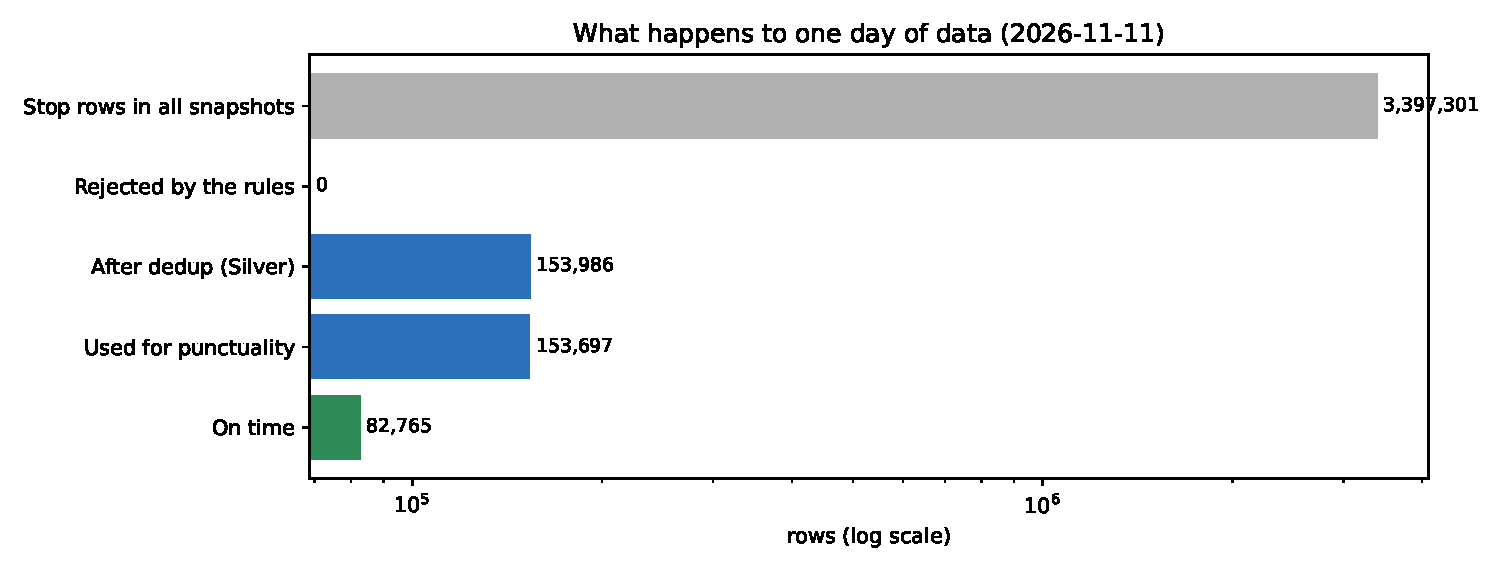
\includegraphics[width=\linewidth]{3_silver_funnel.pdf}
  \caption{One day through Silver.}
  \label{fig:funnel}
\end{subfigure}\hfill
\begin{subfigure}[b]{0.49\linewidth}\centering
  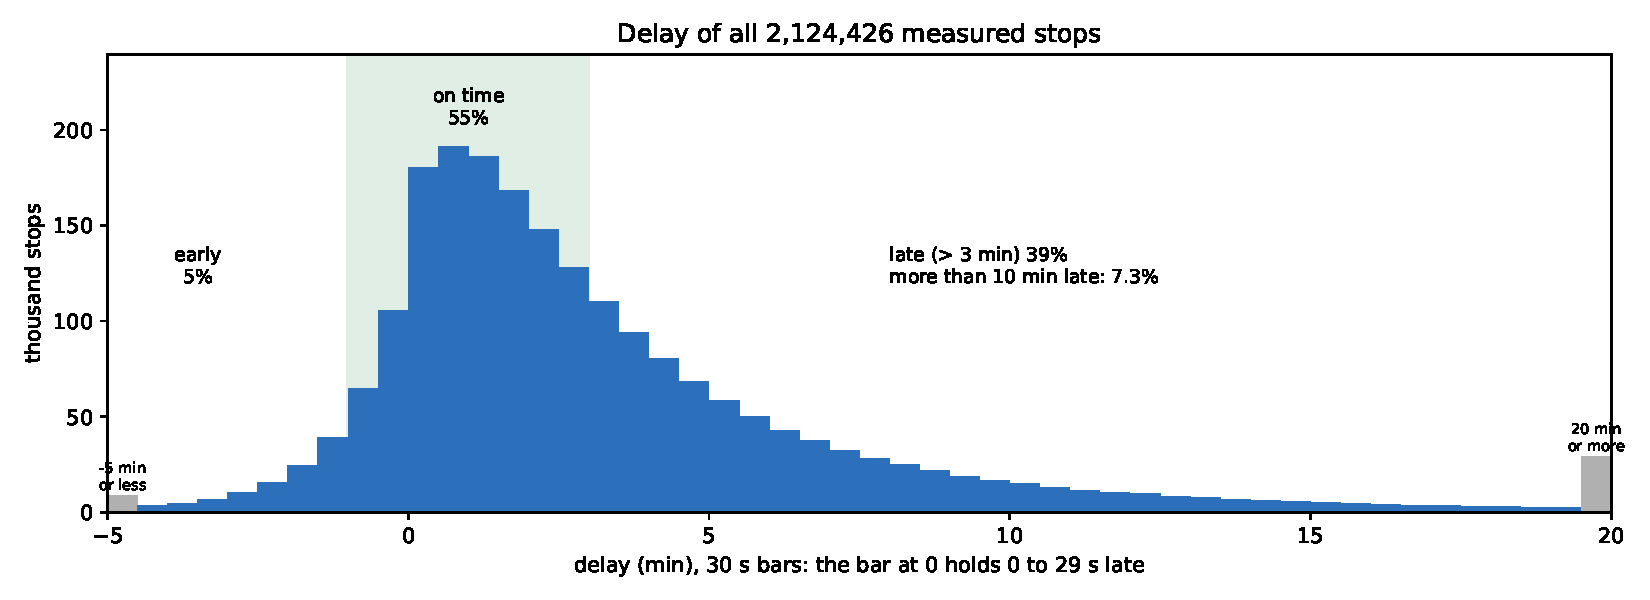
\includegraphics[width=\linewidth]{8_delay_distribution.pdf}
  \caption{Delay of all measured stops.}
  \label{fig:dist}
\end{subfigure}
\caption{Silver quality.}
\end{figure}

\begin{figure}[t]
\centering
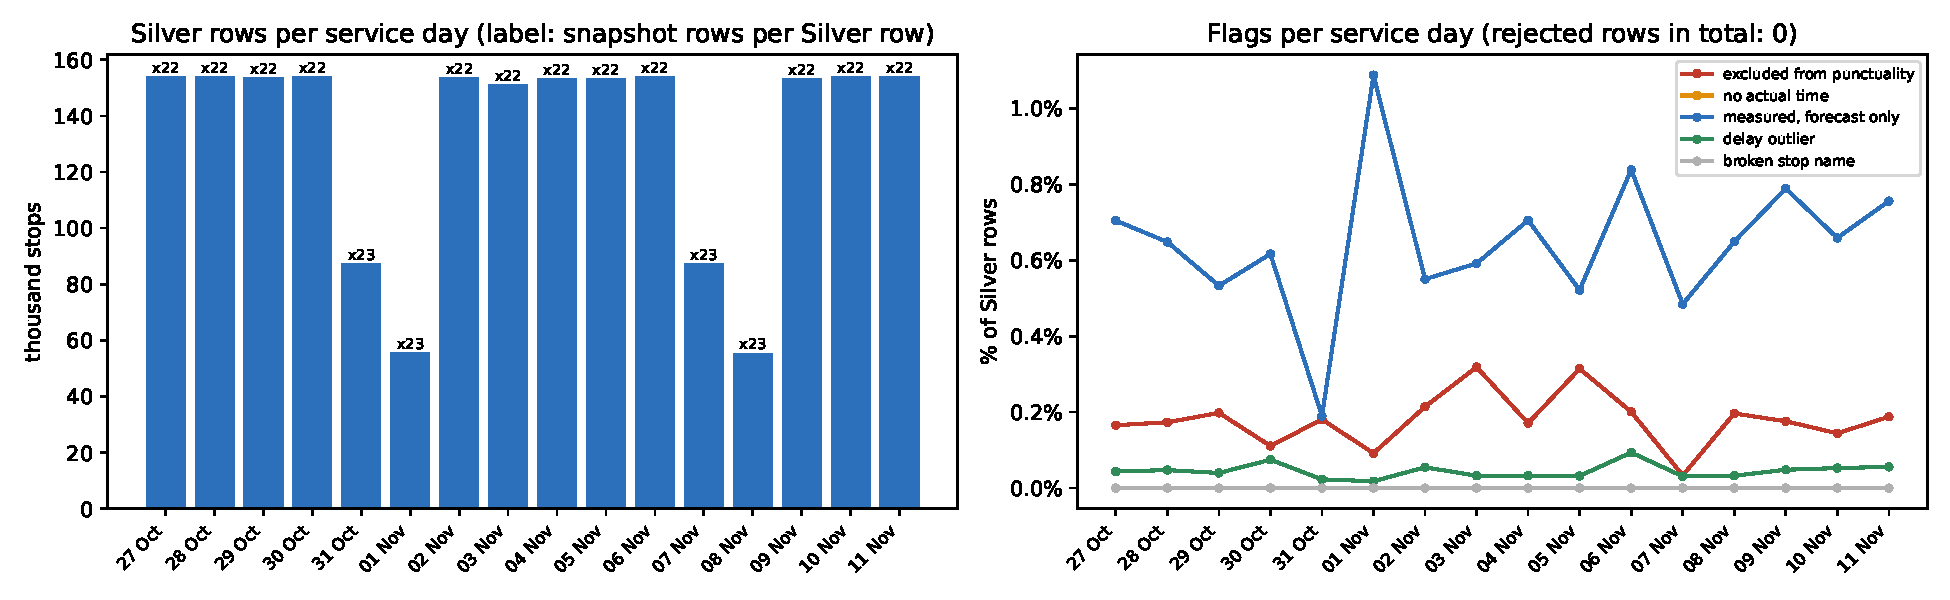
\includegraphics[width=0.85\linewidth]{7_quality_per_day.pdf}
\caption{Silver rows and flags per service day, from the quality table.}
\label{fig:quality}
\end{figure}

\section{Gold}

Silver has about 150k rows a day, while the question needs a few numbers per line, hour and
stop. Gold has two tables partitioned by \code{service\_date}:
\code{punctuality\_by\_line\_hour} and \code{punctuality\_by\_stop}.

On time means between 1 minute early and 3 minutes late. We use the departure delay, or the
arrival delay at the last stop since it has no departure. The hour is the planned time in
Europe/Oslo, converted before grouping, otherwise 8 o'clock would show up as 7. Stops are
grouped by \code{stop\_id} because some lines send no stop names.

Each row stores counts (\code{calls}, \code{measured\_calls}, \code{on\_time\_calls},
\code{late\_calls}, \code{early\_calls}, \code{cancelled\_calls}) as well as the shares,
\code{avg\_delay\_s} and \code{p90\_delay\_s}. Shares cannot be averaged across days, but
counts can be summed and divided again, so any period gives the exact share. The average
delay has to be weighted by \code{measured\_calls} and p90 has to be recomputed from Silver.
We use \code{percentile\_approx} because an exact percentile needs a full sort.

Line numbers come from Entur's Journey Planner. The \code{lines} step only asks about line
ids that are new in Silver, so most nights it makes no API call, and old rows keep their
names. The table has a few hundred rows, so Gold uses a broadcast left join; a line without
a name still counts.

Before writing, Gold checks two things:

\begin{lstlisting}[caption={Gold check in \code{gold/build.py} (shortened).}]
problems = [f"{d}: only {n} rows" for d, n in day_counts if n < 20_000]
# every Silver row must end up in exactly one group of each table
if line_hour_calls != silver_rows or stop_calls != silver_rows:
    problems.append("counts do not match")
if not problems:
    line_hour.write.mode("overwrite").partitionBy("service_date").parquet(...)
\end{lstlisting}

The 20{,}000 rows catch missing data (a Sunday has about 55k). The count check catches bugs
in Gold itself; for example a line listed twice in the names table would double that line
in the join. If something fails, nothing is written, the old Gold stays, the step exits with
an error and a \code{failed} line goes to \code{gold/\_status/status.jsonl}. We query Gold
with Spark SQL in \code{scripts/gold\_report.py}:

\begin{lstlisting}[language=SQL, caption={Least punctual lines.}]
SELECT line, sum(on_time_calls) / sum(measured_calls) AS on_time_share
FROM line_hour GROUP BY line ORDER BY on_time_share LIMIT 10
\end{lstlisting}

\section{Testing, deployment and runs}
\label{sec:lifecycle}

We work on feature branches, open a PR to \code{dev}, and later merge \code{dev} into
\code{main}. \code{tests.yml} runs ruff and 83 pytest tests on GitHub's own machines for
every push and PR. The repo is public, so we did not want PR code running on our VMs; the
self-hosted runners only run merged code. A merge to \code{dev} deploys to the dev VM and a
merge to \code{main} deploys to prod (\code{git pull} and \code{pip install}).

\code{pipeline.yml} runs at 03:17 UTC on the prod runner, or by hand for any day on dev or
prod. Bronze stays on cron because it needs exact timing. Silver and Gold can start late,
and running them in Actions gives us logs, history and a red or green status. The first
scheduled runs started up to 7.5 hours late; moving from 04:00 to 03:17 helped, since GitHub
delays full-hour schedules the most. At the end the workflow writes a summary to the run page
(Bronze runs, Silver rows, Gold status), even after a failure. On prod the run also turns red
with fewer than 270 of 288 valid snapshots, because the 20k check alone would let a half day
through. All decisions are written down with date, owner and reason in
\code{docs/decisions.md}.

\begin{figure}[t]
\centering
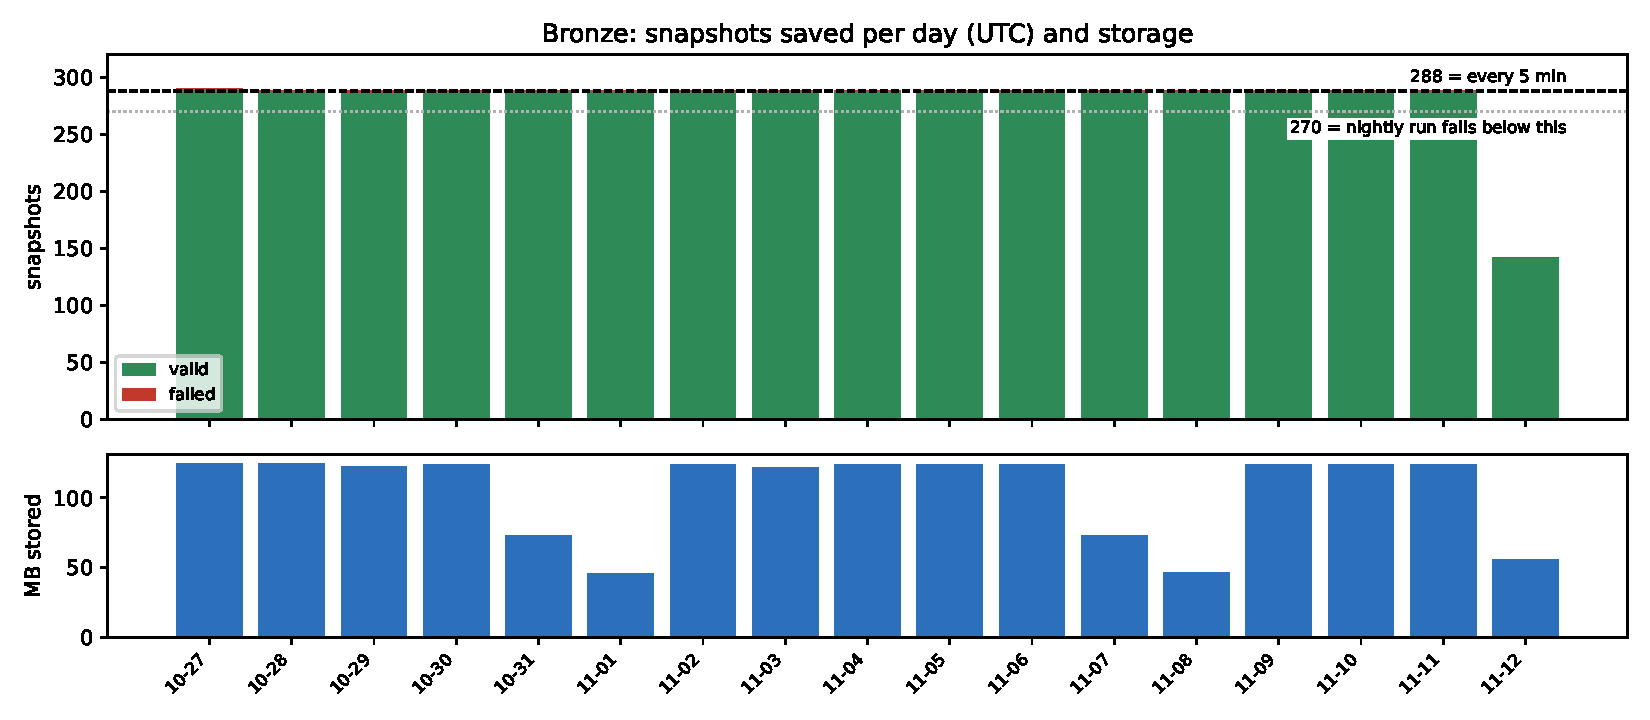
\includegraphics[width=0.8\linewidth]{6_bronze_health.pdf}
\caption{Bronze snapshots saved per day (UTC) and storage used.}
\label{fig:bronze}
\end{figure}

\section{Performance}

We timed one day (4 Nov) on prod with different settings and read the stage times from the
Spark event logs. We ran the baseline twice (310 and 313\,s), so about 3\,s is noise.

\begin{table}[h]
\centering\small
\begin{tabular}{lrr}
\toprule
Change & Before & After \\
\midrule
Gold, shuffle partitions 200 $\rightarrow$ 8 & 28\,s, 1{,}639 tasks & 17\,s, 91 tasks \\
Silver, any shuffle setting & 299--314\,s & no change \\
Silver, 1 / 2 / 3 service days & \multicolumn{2}{r}{308 / 408 / 516\,s} \\
\bottomrule
\end{tabular}
\caption{Measured run times.}
\label{tab:perf}
\end{table}

Gold only groups about 150k rows a day, so 200 shuffle partitions were mostly overhead. AQE
is on by default but did not merge them (same number of tasks with it on or off), so we set
8 in \code{start\_spark}.

Silver did not change at all. The dedup shuffle takes 3 to 8\,s; the rest is Python: parsing
864 XML files (about 137\,s), turning the rows into a DataFrame (about 100\,s) and a second
pass that counts unparseable times (about 27\,s). Spark settings cannot help with that. Each
extra Bronze day costs about 100\,s, so the extra day on each side is around two thirds of a
nightly run, since every file gets parsed on three different nights. The obvious fix is to
parse each file once and store the result. We did not do it before the deadline because a
run takes about 5 minutes, which is fine for a nightly job.

\begin{figure}[t]
\centering
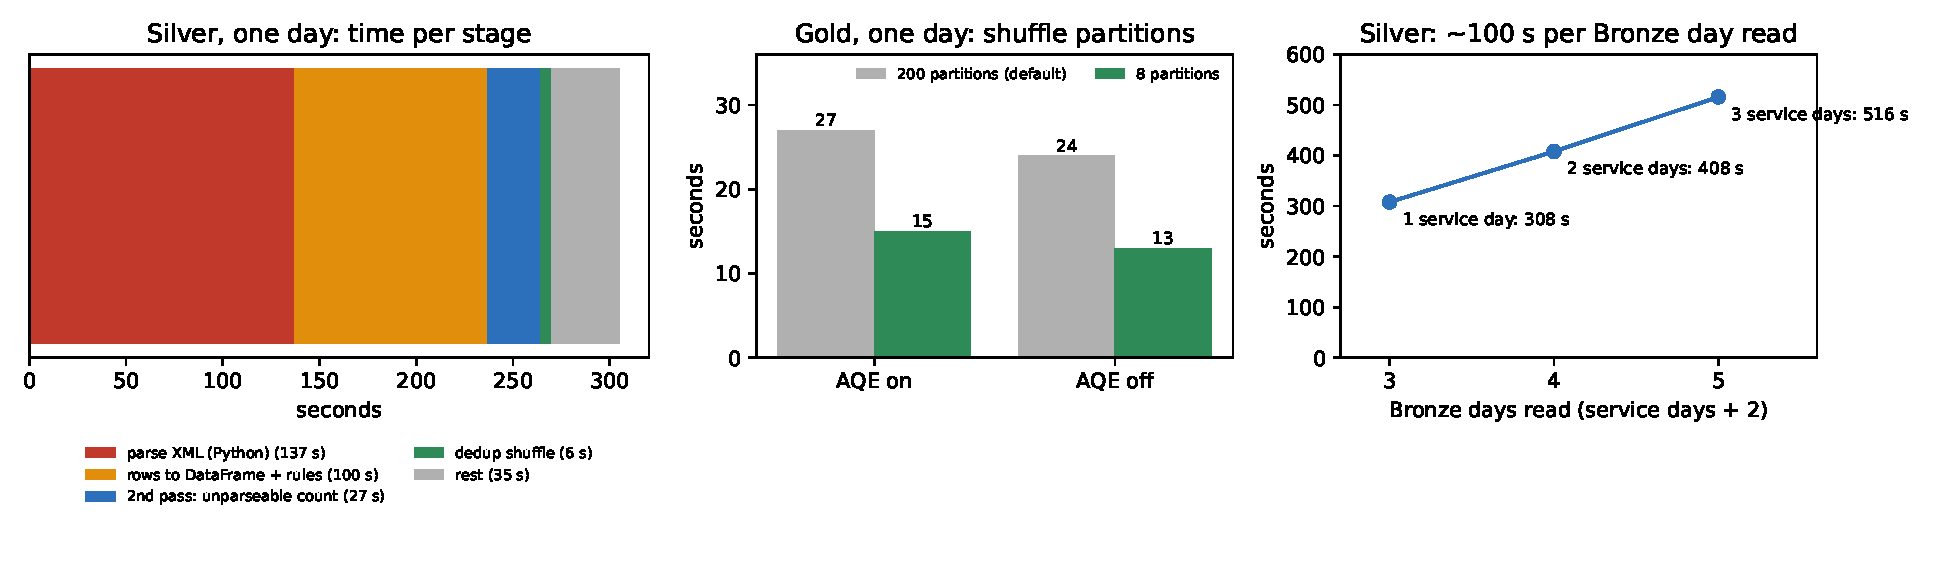
\includegraphics[width=0.85\linewidth]{5_performance.pdf}
\caption{Time per stage in Silver and Gold for one day.}
\label{fig:perf}
\end{figure}

\section{Results}

A weekday gives about 153{,}000 stops, a Saturday 87k and a Sunday 55k. From 27 Oct to
10 Nov Silver has 1{,}974{,}429 rows. About 55\% of measured stops are on time. The afternoon
is the worst: around 15:00 only about 33\% are on time (Figure~\ref{fig:heatmap}). The worst
line is X39 with about 15\%, an express line with three route variants between Stavanger,
Ålgård and Gjesdal (Figure~\ref{fig:lines}). Weekdays stay between about 51\% and 57\%.
Sundays are clearly better (65\% and 69\%), with about a third of the weekday traffic, while
Saturdays are only slightly better than weekdays (Figure~\ref{fig:trend}).

To check the numbers we rely on the Gold count check in every run, on unit tests for the
rules and the dedup order, and on \code{scripts/check\_gold.py}, which follows one trip by
hand from the raw XML to Silver.

\begin{figure}[t]
\centering
\begin{subfigure}[b]{0.52\linewidth}\centering
  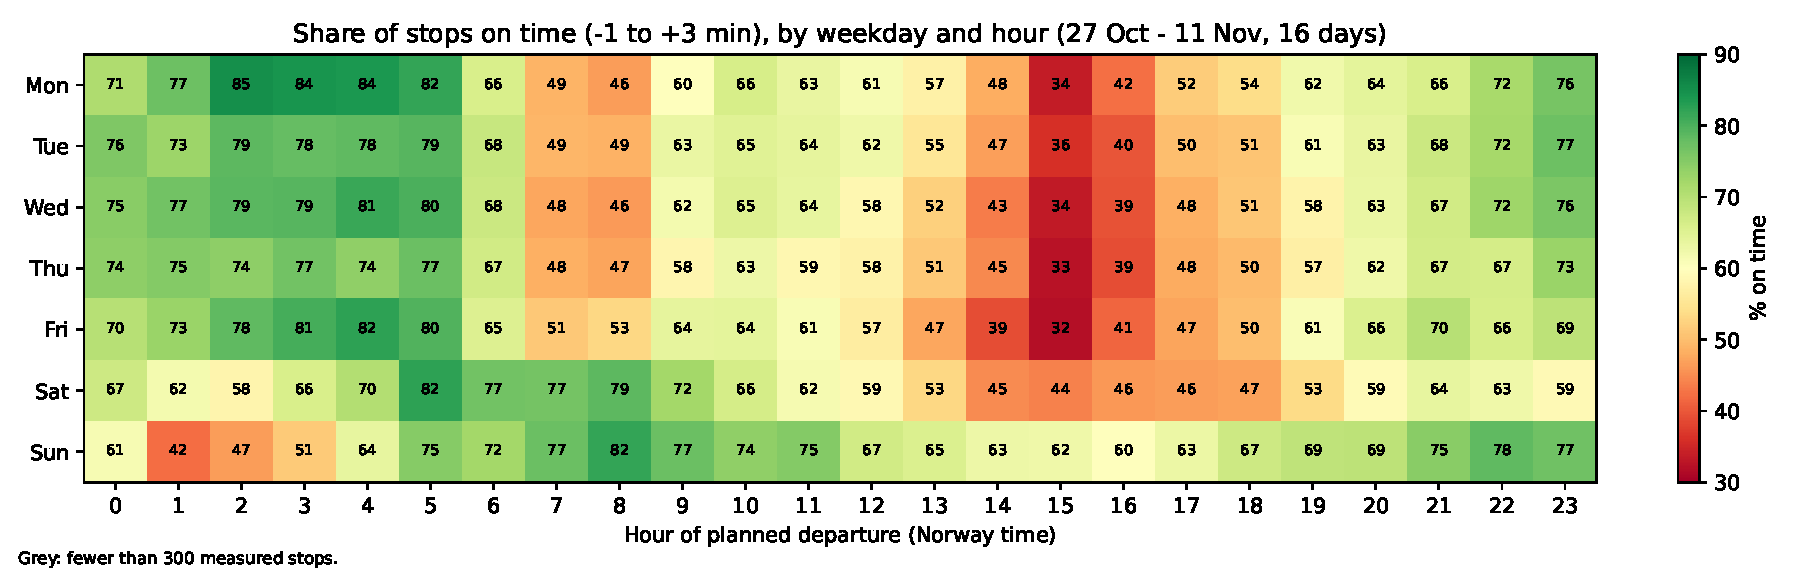
\includegraphics[width=\linewidth]{1_heatmap_weekday_hour.pdf}
  \caption{On-time share by weekday and hour (Oslo time).}
  \label{fig:heatmap}
\end{subfigure}\hfill
\begin{subfigure}[b]{0.46\linewidth}\centering
  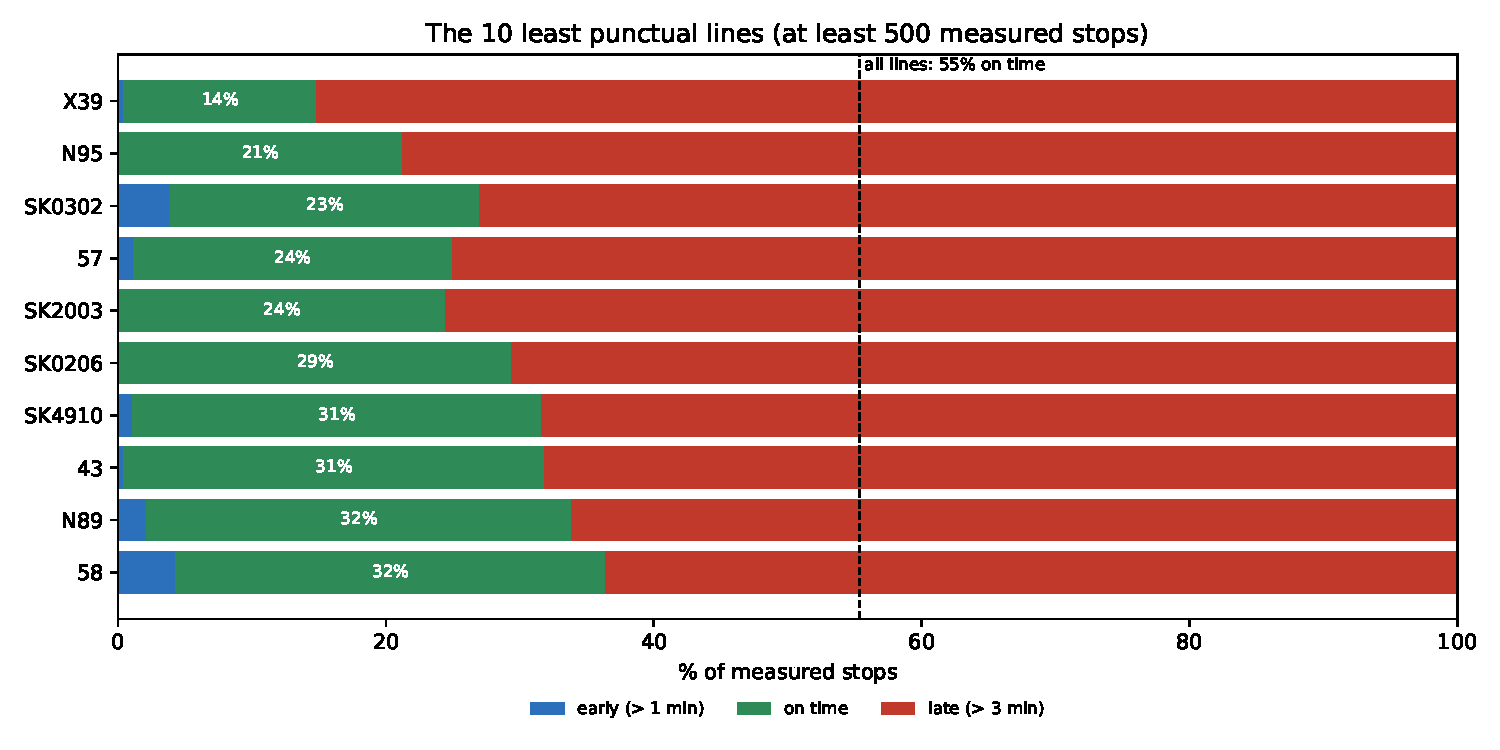
\includegraphics[width=\linewidth]{2_worst_lines.pdf}
  \caption{Least punctual lines.}
  \label{fig:lines}
\end{subfigure}
\caption{Gold results.}
\end{figure}

\begin{figure}[t]
\centering
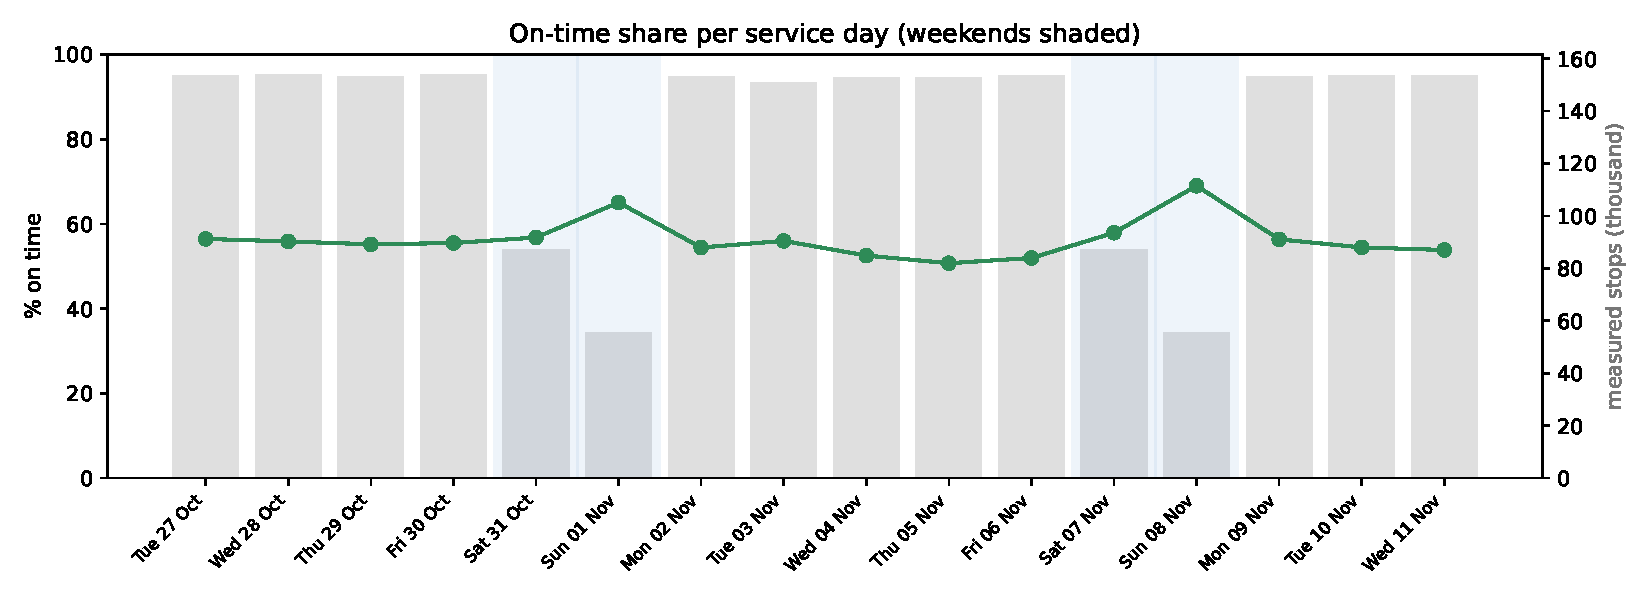
\includegraphics[width=0.85\linewidth]{9_daily_trend.pdf}
\caption{On-time share per service day (weekends shaded).}
\label{fig:trend}
\end{figure}

\section{Reflection}

Most of our decisions came from a measurement: the polling interval, the outlier limits,
keeping predicted stops, the shuffle partitions. Planning for reruns early (partition
overwrite, the extra days, a stable dedup order) made backfills and fixes easy later.
Flagging instead of rejecting meant we could still count cancellations and change the delay
limits without rebuilding Bronze.

Some things went wrong. Fetching from both cron and Actions gave us duplicates and reruns
that did not match. The first Silver run on prod ran out of memory. Our first 50\,GB volume
got stuck in OpenStack while resizing, which left a 45-minute gap on 26 Oct, before the real
collection started. All of these are fixed and documented.

The main limitations:
\begin{itemize}
  \item One VM collects the data. If it is down, those snapshots are lost for good; a second
        collector or a backup to object storage would fix that.
  \item Trips that never appear in the feed are not counted. GTFS would let us count them.
  \item 0.7\% of stops use a predicted time. The effect is small (0.05 points) but not zero.
  \item Silver parses each Bronze file three times and is limited by Python.
  \item \code{avg\_delay\_s} and \code{p90\_delay\_s} cannot simply be added over days.
  \item \code{read\_rows} in \code{silver/build.py} is only used by tests and repeats the
        Spark path; the tests should call \code{read\_file} instead.
\end{itemize}

What we take away: the slow part was Python, not Spark, and we only saw that in the event
logs. And with a live source, collection is what matters most. Silver and Gold can always be
rerun, a missed snapshot cannot. Next we would parse each file once, add GTFS for missing
trips, and build a small dashboard on top of Gold.

\section*{Who did what}

Tommaso: repository, self-hosted runners, GitHub Actions workflows, \code{flatten},
\code{standardize}, \code{dedup}. Oliwier: OpenStack setup, Bronze ingestion and the
retention test, rules, quality table, Gold, line names, performance measurements. Both:
design decisions, code reviews and \code{docs/decisions.md}.

% TODO: say how AI tools were used, as agreed in the group.

\small
\begin{thebibliography}{9}
\bibitem{entur} Entur. \emph{Real-time data (SIRI) API}.
  \url{https://developer.entur.org/pages-real-time-api}
\bibitem{jp} Entur. \emph{Journey Planner API v3}.
  \url{https://developer.entur.org/pages-journeyplanner-journeyplanner}
\bibitem{nlod} Norwegian Licence for Open Government Data (NLOD) 2.0.
  \url{https://data.norge.no/nlod/en/2.0}
\bibitem{spark} Apache Spark documentation, \emph{Performance Tuning}.
  \url{https://spark.apache.org/docs/latest/sql-performance-tuning.html}
\bibitem{repo} Project repository.
  \url{https://github.com/tommasofacchin/rogaland-transit-medallion}
\end{thebibliography}

\end{document}
